\documentclass[a4paper,11pt]{article}
\usepackage[margin=2cm]{geometry}
\usepackage{amsmath}
\usepackage{natbib}
\usepackage{graphicx}
\usepackage{setspace}
\usepackage{multirow}
\usepackage{datetime}

\usepackage{authblk}
%\usepackage{chngcntr}

\usepackage{tabularx}
%\usepackage{mathabx}
\usepackage{subfigure}
\usepackage{fancyheadings}
\usepackage[titletoc]{appendix}
\usepackage{rotating}
\usepackage{bm}
\usepackage{courier}
\usepackage{lineno}

\bibliographystyle{plainnat}

\DeclareGraphicsExtensions{.pdf,.png,.jpg}
\graphicspath{{../img/}}

\usepackage{color, colortbl}
\definecolor{Gray}{gray}{0.6}
\newcommand{\red}[1]{\textcolor{red}{#1}}
\newcommand{\graynew}[1]{\textcolor{Gray}{#1}}

\usepackage{cleveref}

\def\imagetop#1{\vtop{\null\hbox{#1}}}

\usepackage{etoolbox}%Italicsreferences
\makeatletter
\patchcmd{\NAT@test}{\else\NAT@nm}{\else\NAT@nmfmt{\NAT@nm}}{}{}
\let\NAT@up\itshape
\makeatother


\title{Notes}
\date{\today}

\author[1]{Adina E. Pusok}
\affil[1]{\small Depart. of Earth Sciences, University of Oxford, UK}
\affil[*]{\small Corresponding author: adina.pusok@earth.ox.ac.uk}

\begin{document}
\maketitle

%\tableofcontents
%\newpage
\pagestyle{fancyplain}
\rhead[\fancyplain{}{\slshape \rightmark}]{\thepage}
%\lhead{PUSOK ET AL.}
%\lhead[\thepage]{\fancyplain{}%
%{\slshape \leftmark}}
\cfoot{}

%\doublespacing

%% ------------------------------------------------------------------------ %%
%  MAIN BODY
%% ------------------------------------------------------------------------ %%

%\linenumbers
%\begin{abstract}
%\end{abstract}

\section{Theoretical Framework}
The governing equations in geodynamics generally represent conservation of mass, momentum and energy of the form:
\begin{equation}
 \text{Input} + \text{Generation} = \text{Output} + \text{Accumulation} \ + \text{Consumption} 
\end{equation}

\subsection{Single-phase Stokes Flow}
The equations for conservation of mass and momentum (Stokes equations), assuming incompressibility and neglecting thermal diffusion, are given by:

\begin{align}
\nabla \cdot \bm{\sigma}+\rho \textbf{g} &= 0 \\
\nabla \cdot \textbf{v} &= 0,
\end{align}
where $\bm{\sigma}= -P + \bm{\tau}$ is the total stress tensor with $P$ the pressure and $\bm{\tau}$ the deviatoric stress tensor, $\rho$ the fluid density, $\textbf{g}$ the gravitational acceleration and $\textbf{v}$ the velocity. The deviatoric stress tensor can be expressed as:
\begin{align}
\bm{\tau} &= 2\eta\bm{\dot{\varepsilon}} \\
\bm{\dot{\varepsilon}} &= \frac{1}{2}\left(\nabla \textbf{v}+\nabla\textbf{v}^T\right),
\end{align}
where $\bm{\dot{\varepsilon}}$ is the strain rate tensor and $\eta$ is the effective viscosity (constant for linear viscous formulation, non-linear for visco-elasto-plastic rheology).

The momentum equation then becomes:
\begin{align}
\nabla \cdot \bm{\tau}  -  \nabla P +\rho \textbf{g} &= 0 \\
-\nabla P + \nabla \cdot \eta\left(\nabla \textbf{v}+\nabla\textbf{v}^T\right)+\rho \textbf{g} &= 0
\end{align}

So the system of Stokes equations to be solved is:
\begin{align}
\nabla \cdot \textbf{v} &= 0 \label{eq:vecmass}\\
-\nabla P + \nabla \cdot \eta\left(\nabla \textbf{v}+\nabla\textbf{v}^T\right)+\rho \textbf{g} &= 0 \label{eq:vecmomm}
\end{align}

\textbf{Partial derivative form}

For finite difference discretization, sometimes it is easier (and more intuitive) to write the equations in partial derivative form. The equations above can be written as:

\begin{eqnarray}
\frac{\displaystyle \partial v_{i}}{\displaystyle \partial x_i} &= 0 \\
\frac{\displaystyle \partial \sigma_{ij}}{\displaystyle \partial x_j} + \rho g_i &= 0,\\
\end{eqnarray}
where $i,j$ represent spatial directions following the Einstein summation convention, $\sigma_{ij} = -P + \tau_{ij}$ is the total stress tensor with $P = -\sigma_{ij}/3$ the pressure and $\tau_{ij}$ the deviatoric stress tensor, $\rho$ the fluid density, $g_i$ the gravitational acceleration, $v_i$ the velocity and $x_i$ the spatial coordinate. The constitutive equations for the deviatoric stress tensor is $\tau_{ij} = 2\eta\dot{\varepsilon}_{ij}$, and for the deviatoric strain rate tensor $\dot{\varepsilon}_{ij}$:
\begin{align}
\dot{\varepsilon}_{ij} = \frac{1}{2}\left(\frac{\partial v_i}{\partial x_j}+\frac{\partial v_j}{\partial x_i}\right)
\end{align}

Rewriting the momentum equation for $x-$ and $z-$ components and $g_i = [0,0,-g]$, we have:

\begin{align}
\frac{\displaystyle \partial \sigma_{xx}}{\displaystyle \partial x}+\frac{\displaystyle \partial \sigma_{xz}}{\displaystyle \partial z} &= 0 \\
\frac{\displaystyle \partial \sigma_{zx}}{\displaystyle \partial x}+\frac{\displaystyle \partial \sigma_{zz}}{\displaystyle \partial z}-\rho g &= 0,
\end{align}
where 
\begin{align}
\sigma_{xx} &= -P + 2\eta\frac{\displaystyle \partial v_x}{\displaystyle \partial x}\\ 
\sigma_{zz} &= -P + 2\eta\frac{\displaystyle \partial v_z}{\displaystyle \partial z} \\
\sigma_{xz} = \sigma_{zx} &= \eta\left(\frac{\displaystyle \partial v_x}{\displaystyle \partial z}+\frac{\displaystyle \partial v_z}{\displaystyle \partial x}\right) 
\end{align}

Substituting the above equations leads to extended Stokes equations:

\begin{align}
\frac{\displaystyle \partial v_x}{\displaystyle \partial x}+\frac{\displaystyle \partial v_z}{\displaystyle \partial z} &= 0  \label{eq:mass}\\
& \nonumber \\ 
-\frac{\displaystyle \partial P}{\displaystyle \partial x}+2\frac{\displaystyle \partial}{\displaystyle \partial x}\left(\eta\frac{\displaystyle \partial v_x}{\displaystyle \partial x}\right)+\frac{\displaystyle \partial}{\displaystyle \partial z}\left(\eta\left(\frac{\displaystyle \partial v_x}{\displaystyle \partial z}+\frac{\displaystyle \partial v_z}{\displaystyle \partial x}\right)\right) &= 0  \label{eq:momm1}\\
&\nonumber  \\
-\frac{\displaystyle \partial P}{\displaystyle \partial z}+2\frac{\displaystyle \partial}{\displaystyle \partial z}\left(\eta\frac{\displaystyle \partial v_z}{\displaystyle \partial z}\right)+\frac{\displaystyle \partial}{\displaystyle \partial x}\left(\eta\left(\frac{\displaystyle \partial v_x}{\displaystyle \partial z}+\frac{\displaystyle \partial v_z}{\displaystyle \partial x}\right)\right) - \rho g &= 0  \label{eq:momm2}
\end{align}

The unknown variables are: $v_x$, $v_z$ and $P$. 

\subsection{Analytical solutions to Stokes equations: Corner flow}
Based on \citet{Spiegelman1987,Turcotte2014} - (Geodynamics 3rd ed).\\

We can derive analytical solutions to Stokes equations (Eq. \ref{eq:mass}-\ref{eq:momm2}), if we assume no buoyancy ($\rho g =0$) and constant viscosity ($\eta = \eta_0$). Using the constitutive equation to replace the terms $\frac{\partial^2 v_x}{\partial x\partial z}$ and $\frac{\partial^2 v_z}{\partial x\partial z}$, we can write the momentum equations as:

\begin{align}
\frac{\displaystyle \partial P}{\displaystyle \partial x}&=\eta_0\left(\frac{\displaystyle \partial^2 v_x}{\displaystyle \partial x^2} + \frac{\displaystyle \partial^2 v_x}{\displaystyle \partial z^2}\right) \label{eq:momm1-sim}\\
&\nonumber  \\
\frac{\displaystyle \partial P}{\displaystyle \partial z}&=\eta_0\left(\frac{\displaystyle \partial^2 v_z}{\displaystyle \partial x^2} + \frac{\displaystyle \partial^2 v_z}{\displaystyle \partial z^2}\right) \label{eq:momm2-sim}
\end{align}

Or in vector form:
\begin{align}
\nabla P = \eta_0\nabla^2\textbf{v} \label{eq:redpressure}
\end{align}

The incompressible continuity equation can be satisfied with a stream function $\psi$, such that:
\begin{align}
\textbf{v} = \nabla\times\psi\hat{\textbf{j}} \label{eq:stream}
\end{align}
or $v_x = \frac{\partial\psi}{\partial z}$ and $v_z = -\frac{\partial\psi}{\partial x}$. Verify continuity equation:
\begin{align}
\frac{\displaystyle \partial v_x}{\displaystyle \partial x}+\frac{\displaystyle \partial v_z}{\displaystyle \partial z} = \frac{\partial^2\psi}{\partial x\partial z}-\frac{\partial^2\psi}{\partial z\partial x} = 0
\end{align}

Replacing eq. \ref{eq:stream} in the momentum equations (\ref{eq:momm1-sim}-\ref{eq:momm2-sim}), then taking the curl to eliminate the pressure gradient, and adding the component equations together, we obtain:
\begin{align}
2\frac{\partial^4\psi}{\partial x^2\partial z^2}+\frac{\partial^4\psi}{\partial x^4}+\frac{\partial^4\psi}{\partial z^4} = 0
\end{align}
or 
\begin{align}
\nabla^4\psi= 0 \label{eq:biharmonic}
\end{align}

Eq. \ref{eq:biharmonic} is called the \textit{biharmonic equation}. \citet{Batchelor2000} (in 1967) gives a similarity solution to the biharmonic equation with corner flow boundary conditions in polar coordinates of the form:
\begin{align}
\textbf{v} = \frac{1}{r}\frac{\partial\psi}{\partial\theta}\hat{\textbf{r}}-\frac{\partial\psi}{\partial r}\hat{\bm{\theta}} \label{eq:velpolar}
\end{align}

And the stream function:
\begin{align}
\psi = r U_0 f(\theta),
\end{align}
where
\begin{align}
f(\theta) = C_1\sin\theta+C_2\theta\sin\theta+C_3\cos\theta+C_4\theta\cos\theta
\end{align}
and $U_0$ is the characteristic velocity, $C_1-C_4$ are constants determined by model and boundary conditions. \citet{Spiegelman1987} give solutions to corner flow for mid-ocean ridge and subduction models. 

\subsubsection{Mid-ocean ridge model \citep{Spiegelman1987}}
The model and boundary conditions are shown in Figure \ref{fig:corner_flow}A with coordinate system (a), and a full derivation is given in Appendix \ref{App:AppendixA}. Let's define the coordinate systems such that:
\begin{align}
x &= r\sin\theta \\
z &= r\cos\theta \\
r &= \sqrt{x^2+z^2}\\
\theta &= \tan^{-1}({x/z}), \theta\in\left[-\frac{\pi}{2},\frac{\pi}{2}\right]
\end{align}

The stream function is:
\begin{align}
\psi = r U_0 (C_1\sin\theta+C_4\theta\cos\theta)
\end{align}
where the coefficients are:
\begin{align}
C_1 &= \frac{\displaystyle 2\sin^2\alpha}{\displaystyle \pi-2\alpha-\sin2\alpha} \\
C_4 &= -\frac{\displaystyle 2}{\displaystyle \pi-2\alpha-\sin2\alpha} 
\end{align}
and $\alpha$ is the wedge angle at mid-ocean ridges. In \citet{Spiegelman1987}, the coefficients are given as $A=C_1$ and $B=-C_4$.

The polar velocity components:
\begin{align}
 v_r&= U_0(C_1\cos\theta+C_4\cos\theta-C_4\theta\sin\theta) \label{eq:vr}\\
v_\theta&= U_0(-C_1\sin\theta-C_4\theta\cos\theta)\label{eq:vtheta}
 \end{align}
 
The cartesian velocity components:
\begin{align}
v_x = v_r\sin\theta + v_\theta\cos\theta\\
v_z = v_r\cos\theta - v_\theta\sin\theta
\end{align}

Pressure:
\begin{align}
P &= \frac{2C_4 U_0 \eta_0}{r}\cos\theta
\end{align}

\subsubsection{Mid-ocean ridge model (Implemented, Figure \ref{fig:corner_flow}A with coordinate system b)}\label{moranalytic}
Define the coordinate systems such that:
\begin{align}
x &= r\sin\theta \\
z &= -r\cos\theta \\
r &= \sqrt{x^2+z^2}\\
\theta &= \tan^{-1}({-x/z})
\end{align}
 
The cartesian velocity components:
\begin{align}
v_x = v_r\sin\theta + v_\theta\cos\theta\\
v_z = -v_r\cos\theta + v_\theta\sin\theta,
\end{align}
where $v_r$ and $v_\theta$ are defined in eq. \ref{eq:vr}-\ref{eq:vtheta}. 

The pressure also stays the same:
\begin{align}
P &= \frac{2C_4 U_0 \eta_0}{r}\cos\theta
\end{align}

\subsubsection{Subduction model}

The stream function with known coefficients \citep{Spiegelman1987} (Figure \ref{fig:corner_flow}B) is:
\begin{align}
\psi = r (C\sin\theta-C\theta\cos\theta+D\theta\sin\theta),
\end{align}
where
\begin{align}
C&=\frac{\displaystyle \beta\sin\beta}{\displaystyle \beta^2-\sin^2\beta} \\
D&=\frac{\displaystyle \beta\cos\beta-\sin\beta}{\displaystyle \beta^2-\sin^2\beta}
\end{align}
and $\beta$ is the angle of subduction.

The polar velocity components:
\begin{align}
 v_r&= \frac{1}{r}\frac{\partial\psi}{\partial\theta} = C\theta\sin\theta+D\sin\theta+D\theta\cos\theta\\
v_\theta&=-\frac{\partial\psi}{\partial r} = -C\sin\theta+C\theta\cos\theta-D\theta\sin\theta
 \end{align}
 
The polar-cartesian system for the subduction model are defined as: $x=-r\cos\theta$ and $z=r\sin\theta$. In this case, the cartesian velocity components are:
\begin{align}
v_x = -v_r\cos\theta + v_\theta\sin\theta\\
v_z = v_r\sin\theta + v_\theta\cos\theta
\end{align}

Pressure:
\begin{align}
P &= -\frac{2}{r}\left(C\cos\theta-D\sin\theta\right)
\end{align}

\textbf{Alternative.} \citet{Turcotte2014} (Geodynamics 3rd Ed., 2014, Ch. 6.11) also derive a corner flow solution for subduction by only using cartesian coordinates (a bit more complicated to work with because it involves derivatives of $\tan^{-1}$). The stream function is defined in this case as:
\begin{align}
\psi = (A_1x+B_1z)+(C_1x+D_1z)\tan^{-1}(z/x)
\end{align}
where the constants $A_1-D_1$ depend on the model and boundary conditions. If $A_1=0, B_1=C, C_1=C, D_1=D$, the model becomes equivalent to the \citet{Spiegelman1987} solution.

% Figure - model setups
\begin{figure}
\begin{center}
\noindent 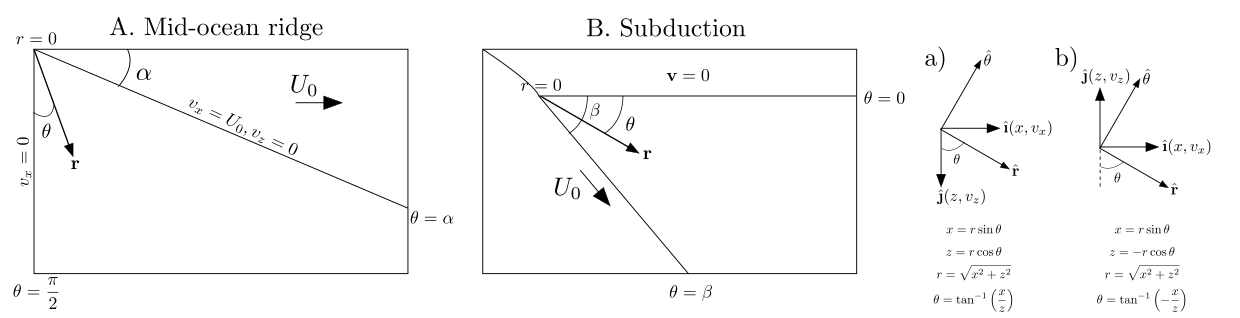
\includegraphics[trim=0mm 0mm 0mm 0mm, clip, width=\textwidth]{corner_flow.pdf} 
\caption{Model setup and boundary conditions for corner flow solutions. A. Mid ocean ridge. B. Subduction. (a)-(b) Different Cartesian-polar coordinate systems.}
\label{fig:corner_flow}
  \end{center}
\end{figure}

\subsection{Constitutive equations}
Rheology. 

\section{Computational Framework}

We solve this using finite differences discretization method on a staggered grid, where the $v_x$ and $v_z$ are located on edges and $P$ in the centre cell.

\subsection{Linear solve}
If $\eta$ is constant (Newtonian viscosity), equations (\ref{eq:mass}-\ref{eq:momm2}) become a linear system of equations written in matrix-vector form as:
\begin{equation}
\textbf{A} \textbf{x} = \textbf{rhs},
\end{equation}
where $\textbf{A}$ is the stiffness matrix, $\textbf{rhs}$ is the right-hand side vector containing the $\rho g$ terms and the boundary conditions, and $\textbf{x} $ is the solution vector. 

One can solve this, by either:
\begin{itemize} 
\item assembling the matrix $\textbf{A}$ and the $\textbf{rhs}$ vector and solving the system as $\textbf{x} = \textbf{A}^{-1}\textbf{rhs}$ (linear solver routines available in most of the linear algebra libraries). The matrix $\textbf{A}$ remains the same for a given system, so can be formed once during a simulation. 
\item minimize residual $r = \textbf{A} \textbf{x} - \textbf{rhs}$, which is matrix free.
\end{itemize}

In case the matrix is assembled, a small modification has to be made to the continuity equation (mass balance):
\begin{equation}
\frac{\displaystyle \partial v_x}{\displaystyle \partial x}+\frac{\displaystyle \partial v_z}{\displaystyle \partial z} = \frac{\displaystyle P}{\displaystyle \gamma}
\end{equation}
where the term $\frac{P}{\gamma}$ is added (assuming incompressibility). This is a "trick" called the penalty method, which ensures that the system of equations does not become ill-posed. $\gamma$ has to be sufficiently large ($\sim 10^4$).

Figure \ref{fig:stokes_ksp} shows the stencil for the linear viscous Stokes case, and a PETSc example of how to solve the system is given in \texttt{./petsc\_examples/stokes\_ksp/}.

% Figure - stokes_ksp
\begin{figure}
\begin{center}
\noindent 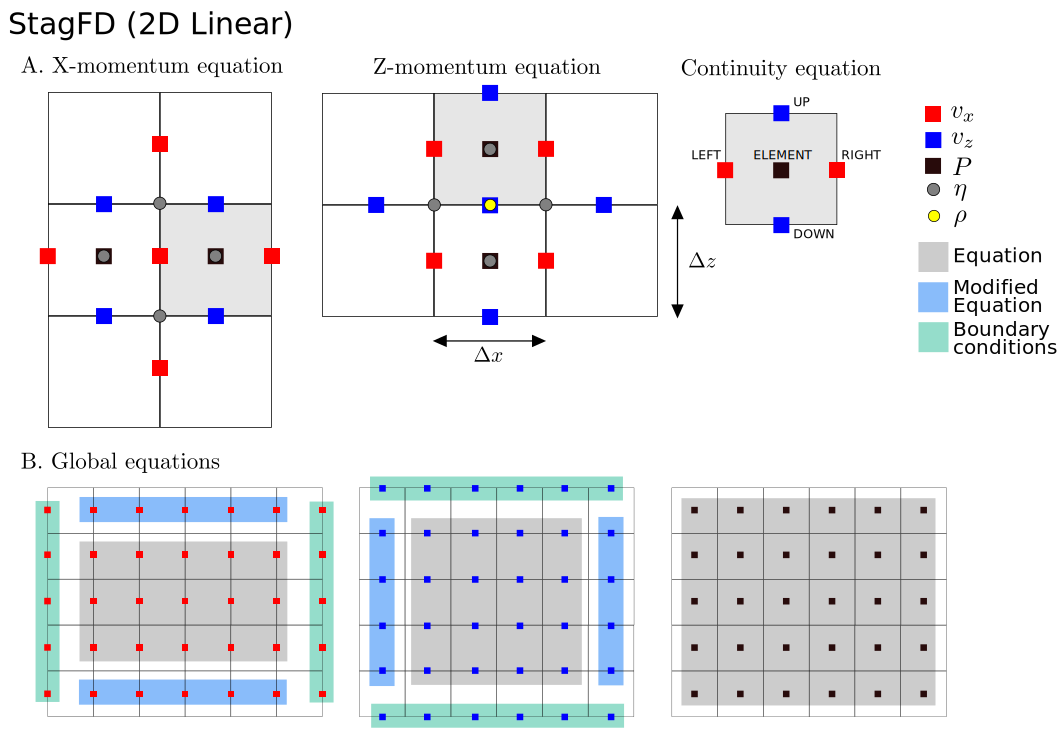
\includegraphics[trim=0mm 0mm 0mm 0mm, clip, width=\textwidth]{dmstag.pdf} 
\caption{Staggered grid finite differences stencils for linear viscous Stokes equations (using the DMStag framework from PETSc).}
\label{fig:stokes_ksp}
  \end{center}
\end{figure}

\subsection{Nonlinear solve}
If $\eta$ is non-linear (depending on P, T, strain rate etc.), equations (\ref{eq:mass}-\ref{eq:momm2}) become a nonlinear system of equations of the form:
\begin{equation}
\textbf{F(x)} = 0.
\end{equation}
When using the Newton method to solve the system, we need to define $\textbf{J(x}_\textbf{k}) = \textbf{F}^\prime\textbf{(x}_\textbf{k})$, which is the Jacobian matrix at the iteration $\textbf{x}_\textbf{k}$. If the viscosity is constant, the Jacobian matrix becomes the same as the stiffness matrix above. PETSc offers more details on how to solve the nonlinear system of equations using SNES.

Figure \ref{fig:stokes_snes} shows the stencil for the nonlinear Stokes case, and a PETSc example of how to solve the system is given in \texttt{./petsc\_examples/stokes\_snes/}.

% Figure - stokes_snes
\begin{figure}
\begin{center}
\noindent 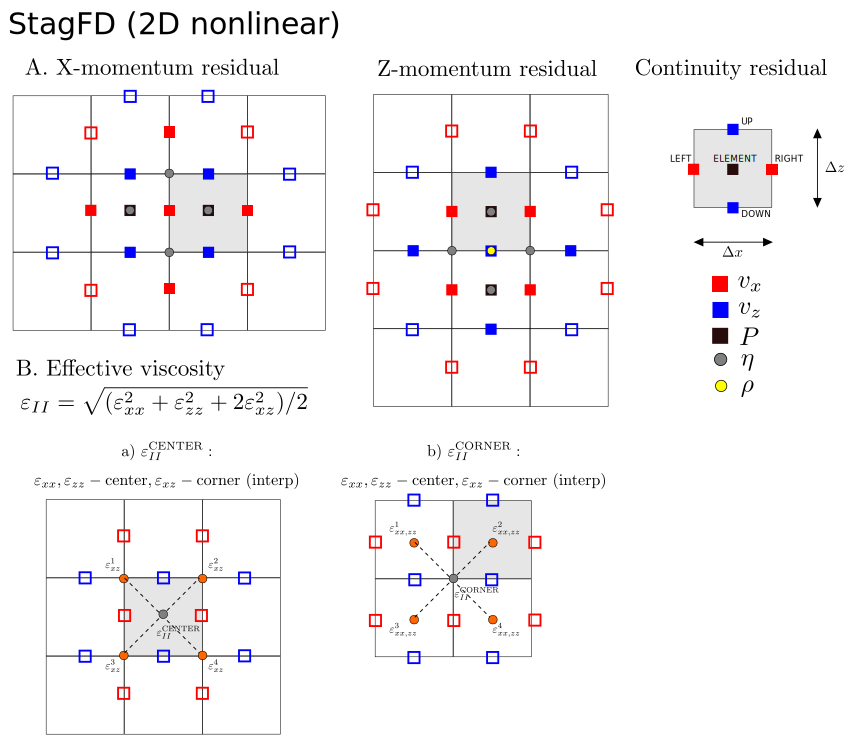
\includegraphics[trim=0mm 0mm 0mm 0mm, clip, width=\textwidth]{dmstag_snes.pdf} 
\caption{Staggered grid finite differences stencils for nonlinear viscous Stokes equations (using the DMStag framework from PETSc).}
\label{fig:stokes_snes}
  \end{center}
\end{figure}

*notes on discretization/implementation

\section{Benchmarks}

\subsection{SolCx \citep{Zhong1996, Moresi1996, Duretz2011}} \label{solcx}
2-D analytical solution of a variable viscous Stokes flow with sharp viscosity jumps. The model domain is defined as $\Omega = [0, 1] \times [0, 1]$. The boundary conditions on all sides of the domain are free-slip, implying that the normal velocity to each wall is zero, and the tangential stress along the wall vanishes. 

The density field is set as:
\begin{equation}
\rho(x,z) = \sin(\pi z) \cos(\pi x)
\end{equation}

And the viscosity field is set as:
\begin{equation}
\eta(x,z) = \left\{\begin{array}{lr}
    \eta_0, &  x \le 0.5\\
    \eta_1, & x > 0.5
  \end{array}\right.
\end{equation}

Internal to the domain, fluid flow is driven by a sinusoidal force given by:
\begin{equation}
F = (0,-\sin(\pi z) \cos(\pi x)^T
\end{equation}

Table \ref{tab:solcx} contains the input parameters for the SolCx model.

% Table - Parameters table eta1,eta2, L, H, xmin, zmin
\begin{table}[h]
\begin{center}
\footnotesize
%\def\arraystretch{0.8}
\begin{tabular}{c c l}
\hline 
Parameter (input)&Value&Comments\\
\hline
L&1&\\
H&1&\\
xmin&0&\\
zmin&0&\\
eta0&1&$\eta_0$\\
eta1&1-$10^6$&$\eta_1$\\
\hline  
\end{tabular}
\caption{SolCx input parameters.}
\label{tab:solcx}
\end{center}
\end{table}

\subsection{Benchmark list}
Tests can be run in \texttt{./StagRidge/tests/} with \texttt{./run\_tests.sh} (requires python) or run each python script individually.

% Table - Benchmarks
\begin{table}[h]
\begin{center}
\footnotesize
%\def\arraystretch{0.8}
\begin{tabular}{l l l l}
\hline 
Name&Input files&Test&Comments\\
\hline
SolCx&\texttt{solcx\_1e0.opts, solcx\_1e6.opts}&\texttt{test\_solcx.py}&Section \ref{solcx}\\
Corner flow (MOR)&\texttt{mor\_isovisc.opts}&\texttt{test\_cornerflow\_mor.py}&Section \ref{moranalytic}\\
\hline  
\end{tabular}
\caption{Benchmark tests}
\label{tab:benchmark}
\end{center}
\end{table}

\textbf{Other Stokes benchmarks}

*SolKz - Revenaugh and Parsons 1987, Underworld
*Rayleigh-Taylor (with free surface) - Kaus et al 2010, Schmeling et al 2008
*Pure shear inclusion test - Schmid and Podladchikov 2003, Schmid 2002, Moulas et al, 2014

Papers using benchmarks and other useful tests for Stokes equations:
Deubelbeiss and Kaus 2008, Schmeling et al. 2008, Gerya 2009, Kaus et al. 2010, Duretz et al. 2011, Dabrowski et 2008, Raess et al 2017, Pusok et al. 2017.

%% ------------------------------------------------------------------------ %%
%  APPENDIX
%% ------------------------------------------------------------------------ %%
\appendix

\section{Corner flow analytical solution for Mid-ocean ridges (Full derivation)} \label{App:AppendixA}

The biharmonic equation:
\begin{align}
\nabla^4\psi= 0
\end{align}

\citet{Batchelor2000} gives a similarity solution to the biharmonic equation with corner flow boundary conditions in polar coordinates of the form:
\begin{align}
\textbf{v} = \frac{1}{r}\frac{\partial\psi}{\partial\theta}\hat{\textbf{r}}-\frac{\partial\psi}{\partial r}\hat{\bm{\theta}} \label{eq:velpolar}
\end{align}

And the stream function:
\begin{align}
\psi = r U_0 f(\theta),
\end{align}
where
\begin{align}
f(\theta) &= C_1\sin\theta+C_2\theta\sin\theta+C_3\cos\theta+C_4\theta\cos\theta \\
f'(\theta) &= C_1\cos\theta+C_2\sin\theta+C_2\theta\cos\theta-C_3\sin\theta+C_4\cos\theta-C_4\theta\sin\theta 
\end{align}
and $U_0$ is the characteristic velocity, $C_1-C_4$ are constants determined by model and boundary conditions. 

From eq. \ref{eq:velpolar}, we can write:
\begin{align}
\textbf{v} = v_r\hat{\textbf{r}}+v_\theta\hat{\bm{\theta}} = v_x\hat{\textbf{i}}+v_z\hat{\textbf{j}} \label{eq:vgen}
\end{align}
where 
\begin{align}
v_r= \frac{1}{r}\frac{\partial\psi}{\partial\theta} = U_0 f'(\theta)\\
v_\theta=-\frac{\partial\psi}{\partial r} = -U_0 f(\theta). 
\end{align}
We want to find expressions for $C_1-C_4$ and $v_x$, $v_z$ and $P$ for a mid-ocean ridge setup (Figure \ref{fig:corner_flow}A).

Let's define the coordinate systems such that (Figure \ref{fig:corner_flow}a):
\begin{align}
x &= r\sin\theta \\
z &= r\cos\theta \\
r &= \sqrt{x^2+z^2}\\
\theta &= \tan^{-1}({x/z}), \theta\in\left[-\frac{\pi}{2},\frac{\pi}{2}\right]
\end{align}

\subsection{Boundary conditions}

1) $\theta = \frac{\pi}{2}-\alpha, v_x = U_0, v_z = 0$
\begin{align}
v_r= U_0\cos\alpha, f'(\frac{\pi}{2}-\alpha) = \cos\alpha\\
v_\theta=U_0\sin\alpha, f(\frac{\pi}{2}-\alpha) = -\sin\alpha\\
\end{align}

2) $\theta = -(\frac{\pi}{2}-\alpha), v_x = -U_0, v_z = 0$
\begin{align}
v_r= U_0\cos\alpha, f'(-\frac{\pi}{2}+\alpha) = \cos\alpha\\
v_\theta=-U_0\sin\alpha, f(-\frac{\pi}{2}+\alpha) = \sin\alpha\\
\end{align}

The above equations represent a system of 4 equations with 4 unknowns ($C_1-C_4)$. We find:
\begin{align}
C_1 &= \frac{\displaystyle 2\sin^2\alpha}{\displaystyle \pi-2\alpha-\sin2\alpha} \\
C_2 &= 0\\
C_3 &= 0\\
C_4 &= -\frac{\displaystyle 2}{\displaystyle \pi-2\alpha-\sin2\alpha} 
\end{align}

The polar coordinate function and velocity become:
\begin{align}
f(\theta) &= C_1\sin\theta+C_4\theta\cos\theta \\
v_r&= U_0 f'(\theta) = U_0*(C_1\cos\theta+C_4\cos\theta-C_4\theta\sin\theta\\
v_\theta&=-U_0 f(\theta) = U_0*(-C_1\sin\theta-C_4\theta\cos\theta)
\end{align}

\subsection{Cartesian coordinate velocity}
We need to transform the basis polar vectors $\hat{\textbf{r}}$ and $\hat{\bm{\theta}}$ into cartesian basis vectors $\hat{\textbf{i}}(x,v_x)$ and $\hat{\textbf{j}}(z,v_z)$. Let:
\begin{align}
\textbf{r} = x\hat{\textbf{i}}+z\hat{\textbf{j}} = r\sin\theta\hat{\textbf{i}} + r\cos\theta\hat{\textbf{j}}
\end{align}
The basis vectors are defined: 
\begin{align}
\hat{\textbf{r}} = \frac{\frac{d\textbf{r}}{dr}}{\left|\frac{d\textbf{r}}{dr}\right|} = \sin\theta\hat{\textbf{i}} + \cos\theta\hat{\textbf{j}}\\
&\nonumber  \\
\hat{\bm{\theta}} = \frac{\frac{d\textbf{r}}{d\theta}}{\left|\frac{d\textbf{r}}{d\theta}\right|} = \cos\theta\hat{\textbf{i}} - \sin\theta\hat{\textbf{j}}
\end{align}
Therefore, from equation \ref{eq:vgen}, the cartesian components of velocity are:
\begin{align}
v_x = v_r\sin\theta + v_\theta\cos\theta \label{eq:vx}\\
v_z = v_r\cos\theta - v_\theta\sin\theta \label{eq:vz}
\end{align}

It can be easily shown that these expressions satisfy the continuity equation. 

\subsection{Pressure}
The pressure is obtained from equation $\nabla P = \eta_0\nabla^2\textbf{v}$. First, let's calculate some derivatives:
\begin{align}
&\frac{\partial r}{\partial x} = \sin\theta\\
&\frac{\partial r}{\partial z} = \cos\theta\\
&\frac{\partial \theta}{\partial x} = \frac{z}{x^+z^2} = \frac{\cos\theta}{r}\\
&\frac{\partial \theta}{\partial z} = -\frac{x}{x^+z^2} = -\frac{\sin\theta}{r}\\
&\frac{\partial v_r}{\partial r} = 0\\
&\frac{\partial v_\theta}{\partial r} = 0\\
&\frac{\partial v_r}{\partial \theta} = -C_1\sin\theta-2C_4\sin\theta-C_4\theta\cos\theta\\
&\frac{\partial v_\theta}{\partial \theta} = -C_1\cos\theta-C_4\cos\theta+C_4\theta\sin\theta = -v_r
\end{align}

Also, let:
\begin{align}
&\frac{\partial v_x}{\partial r} = M\\
&\frac{\partial v_x}{\partial \theta} = N\\
\end{align}

Then, the X-momentum equation becomes:
\begin{align}
\frac{\displaystyle \partial P}{\displaystyle \partial x}=\eta_0\left(\frac{\displaystyle \partial^2 v_x}{\displaystyle \partial x^2} + \frac{\displaystyle \partial^2 v_x}{\displaystyle \partial z^2}\right) = \eta_0\left(\frac{\partial M}{\partial r} + \frac{1}{r}M +\frac{1}{r^2}\frac{\partial N}{\partial \theta}\right) = \eta_0\left( -\frac{4C_4U_0\sin\theta\cos\theta}{r^2}\right)
\end{align}
after using the chain rule:
\begin{align}
 \frac{\partial}{\partial x}=\frac{\partial r}{\partial x}\frac{\partial}{\partial r}+\frac{\partial \theta}{\partial x}\frac{\partial}{\partial \theta}.
 \end{align}
The solution for pressure is given by:
\begin{align}
P =  \frac{2C_4\eta_0 U_0}{r}\cos\theta.
 \end{align}

%% ------------------------------------------------------------------------ %%
%  BIBLIOGRAPHY
%% ------------------------------------------------------------------------ %%

%\bibliographystyle{apalike}
\bibliography{references}

%\begin{thebibliography}{}
%\end{thebibliography}

\end{document}